\documentclass{beamer}
\mode<presentation>
{
  \usetheme{default}      % or try Darmstadt, Madrid, Warsaw, ...
  \usecolortheme{default} % or try albatross, beaver, crane, ...
  \usefonttheme{default}  % or try serif, structurebold, ...
  \setbeamertemplate{navigation symbols}{}
  \setbeamertemplate{caption}[numbered]
} 

\usepackage[english]{babel}
\usepackage[utf8x]{inputenc}
\usepackage{scrextend}
\usepackage{graphicx}
\usepackage{booktabs}
\usepackage{adjustbox}
\usepackage{marvosym}
\graphicspath{ {E:/faculta/Master/DissertationProject/images/} }

\title[Pres]{An analysis of the relationship between structural and logical\\ dependencies in software systems }
\author{Stana Adelina Diana}
\institute{Computer Science and Engineering Department\\
"Politehnica" University of Timisoara}
\date{June, 2018}

\begin{document}

\begin{frame}
  \titlepage
\end{frame}

% Uncomment these lines for an automatically generated outline.
%\begin{frame}{Outline}
%  \tableofcontents
%\end{frame}
%%%%%%%%%%%%%%%%%%%%%%%%%%%%%%%%%%%%%%%%%%
 \begin{frame}
\frametitle{Dependencies}
\begin{columns}
\begin{column}{0.5\textwidth}
    \begin{center}
     \begin{figure}
	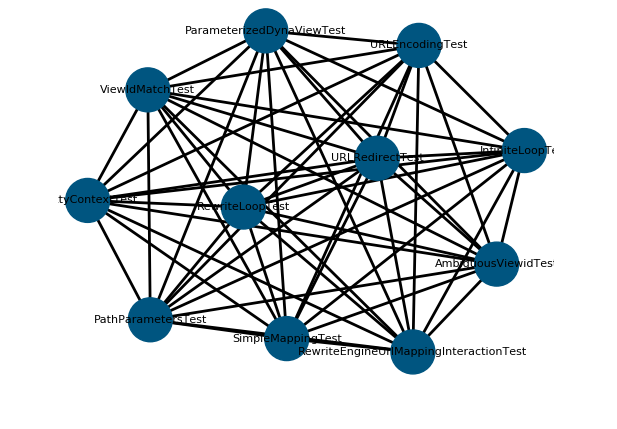
\includegraphics[width=\textwidth]{dependencies.png}
	\caption{\label{fig:your-figure}Dependencies in a project}
     \end{figure}
     \end{center}
\end{column}
\begin{column}{0.5\textwidth}

A  \texttt{dependency} is a relationship that shows that an element, or set of elements, requires other elements for their specification or implementation. [ UML Specification]

\end{column}
\end{columns}
\end{frame}
%%%%%%%%%%%%%%%%%%%%%%%%%%%%%%%%%%%%%%%%%%

 \begin{frame}
\frametitle{Structural dependencies}
\begin{block}{Definition}
Structural dependencies are the result of \it{source code analysis} and can be extracted from : members, call parameters, local variables. 
\end{block}

\begin{center}
     \begin{figure}
	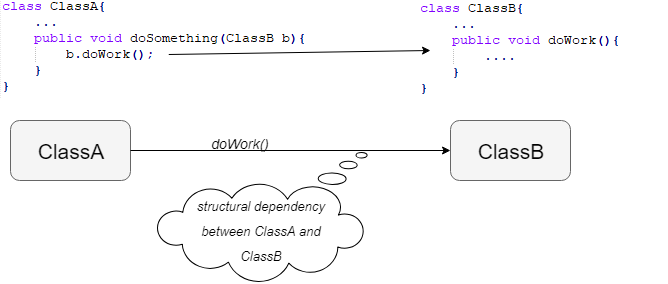
\includegraphics[width=\textwidth]{structural_dep.png}
	\caption{\label{fig:fig}Example of structural dependency between two classes}
     \end{figure}
\end{center}

\end{frame}

%%%%%%%%%%%%%%%%%%%%%%%%%%%%%%%%%%%%%%%%%%%

 \begin{frame}
\frametitle{Logical dependencies}
\begin{block}{Definition}
 Logical dependencies are the result of \it{software history analysis} and can reveal relationships that are not present in the source code code (structural dependencies).
\end{block}

\begin{center}
     \begin{figure}
	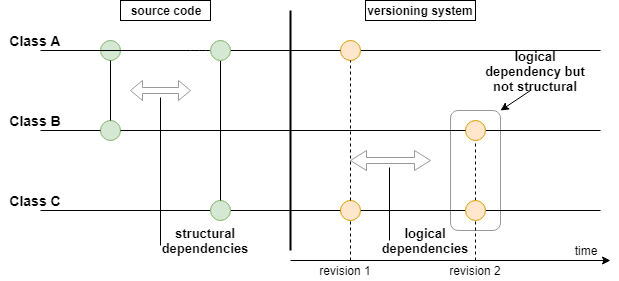
\includegraphics[width=\textwidth]{fig1.png}
	\caption{\label{fig:fig1}Example of logical and structural dependencies}
     \end{figure}
\end{center}

\end{frame}

%%%%%%%%%%%%%%%%%%%%%%%%%%%%%%%%%%%%%%%%%%%
 \begin{frame}
\frametitle{Logical dependencies}
\begin{block}{Research questions}
\vskip 0.3cm
We build logical dependencies based on three questions :\\
\textit{\textbf{Question 1:} How the number of files changed in a commit can influence the logical dependencies of the system?}\\
\textit{\textbf{Question 2:} Considering comment changes as valid changes can lead to additional logical dependencies ? }\\
\textit{\textbf{Question 3:} One occurrence of a logical dependency is enough to consider it as valid ?}\\
\end{block}
\end{frame}

%%%%%%%%%%%%%%%%%%%%%%%%%%%%%%%%%%%%%%%%%%%

 \begin{frame}
\frametitle{Tool for measuring software dependencies}
 In order to answer these research questions, we have built a tool that extracts structural and logical dependencies.
\begin{center}
     \begin{figure}
	\includegraphics[width=\textwidth]{tool2.png}
	\caption{\label{fig:figtool} User Interface}
     \end{figure}
\end{center}

\end{frame}


%%%%%%%%%%%%%%%%%%%%%%%%%%%%%%%%%%%%%%%%%%%

 \begin{frame}
\frametitle{Tool for measuring software dependencies}

\begin{center}
     \begin{figure}
	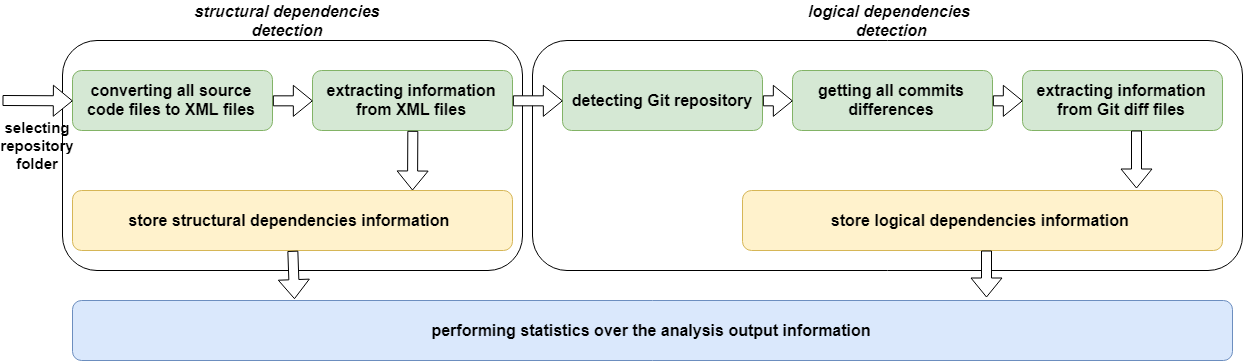
\includegraphics[width=\textwidth]{fig3.png}
	\caption{\label{fig:fig3}Workflow diagram of the tool}
     \end{figure}
\end{center}
\changefontsizes{7.5pt}
The workflow can be delimited by three major steps as it follows:
\begin{itemize}
\item Extracting structural dependencies.
\item Extracting logical dependencies.
\item Processing the information extracted.
\end{itemize}

\end{frame}

%%%%%%%%%%%%%%%%%%%%%%%%%%%%%%%%%%%%%%%%%%%

\begin{frame}
\frametitle{Open source projects studied}
\vskip 0.2cm
\adjustbox{max height=\dimexpr\textheight-5.5cm\relax,
           max width=\textwidth}{
\begin{tabular}{*{5}{l}}
  \toprule
    ID  & Project    & Nr. of classes & Nr. of commits\\
    \midrule
1	&	urSQL	&	41	&	89	&	java	\\
2	&	JavaCoder	&	5	&	11	&	java	\\
3	&	jbandwidthlog	&	14	&	54	&	java	\\
4	&	sjava-logging	&	18	&	62	&	java	\\
5	&	daedalum	&	66	&	29	&	java	\\
6	&	prettyfaces	&	236	&	207	&	java	\\
7	&	jbal	&	102	&	113	&	java	\\
8	&	guavatools	&	237	&	85	&	java	\\
9	&	monome-pages	&	240	&	280	&	java	\\
10	&	kryo	&	309	&	743	&	java	\\
11	&	bitlyj	&	21	&	81	&	java	\\
12	&	slema	&	276	&	368	&	java	\\
13	&	bluecove	&	435	&	1679	&	java	\\
14	&	gp-net-radius	&	25	&	28	&	java	\\
15	&	aima-java	&	833	&	1181	&	java	\\
16	&	powermock	&	966	&	1512	&	java	\\
17	&	restfb	&	757	&	1545	&	java	\\
18	&	Tensorflow	&	1104	&	2386	&	cpp	\\
19	&	mangnum	&	143	&	1728	&	cpp	\\
    \bottomrule
  \end{tabular}}


\end{frame}

%%%%%%%%%%%%%%%%%%%%%%%%%%%%%%%%%%%%%%%%%%%

 \begin{frame}
\frametitle{Experimental results I}

\begin{center}
     \begin{figure}
	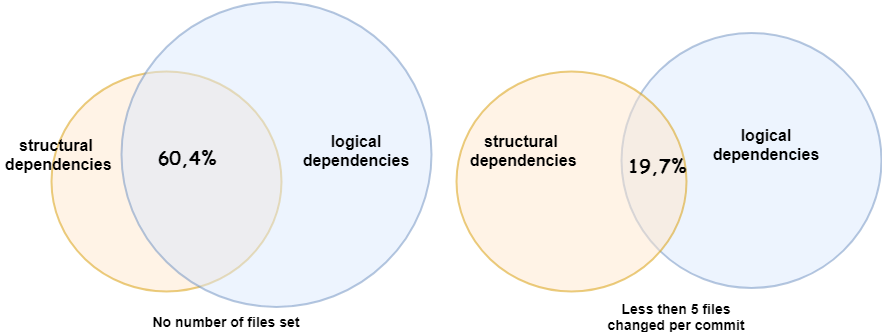
\includegraphics[width=\textwidth]{fig4.png}
	\caption{\label{fig:fig44}Venn diagrams of the overlapping rates with comments taken into consideration as change.}
     \end{figure}
\end{center}
\centering
\adjustbox{max height=\dimexpr\textheight-8.3cm\relax,
           max width=\textwidth}{
\begin{tabular}{*{3}{l}}
    \toprule
       Category & With comments & Without comments  \\
    \midrule
less 5	&	19,7\% &	18,9\%	\\
more 5 less 20	&	31,19\% &	28,7\%\\
more 20	&	31,47\%	&	29,43\%\\
total & 60,4\% &57,28\% \\
    \bottomrule
  \end{tabular}
}
\end{frame}


 \begin{frame}
\frametitle{Experimental results II}

\begin{center}
     \begin{figure}
	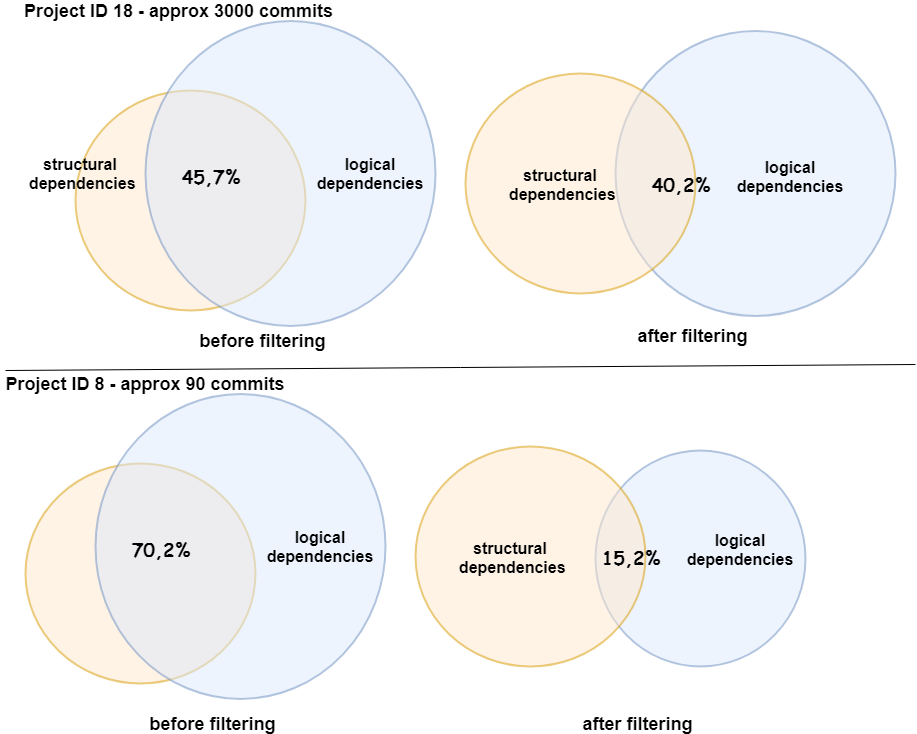
\includegraphics[width=\textwidth]{figvenn3.png}
	\caption{\label{fig:figvenn}Impact of logical dependencies occurrences filtering on projects with different sizes.}
     \end{figure}
\end{center}

\end{frame}

%%%%%%%%%%%%%%%%%%%%%%%%%%%%%%%%%%%%%%%%%%%

 \begin{frame}
\frametitle{Conclusions}
 \begin{itemize}
        \item  Large number of structural dependencies are not doubled by logical \MVRightarrow{} systems partially stable
        \item  + -3\% for comments as a change
        \item The number of changed files taken into consideration influence the results
	\begin{itemize}   
	\item big threshold  \MVRightarrow{} not so relevant logical dependencies
	\item small threshold (5~10)  \MVRightarrow{} more accurate results
    	\end{itemize}
      \item Filtering the logical dependencies after occurrences is good only for projects with a significant number of commits. 
    \end{itemize}
\begin{block}{Future work}
Investigate the cause for the large number of logical dependencies which are not overlapping with structural dependencies.
\end{block}
\end{frame}

%%%%%%%%%%%%%%%%%%%%%%%%%%%%%%%%%%%%%%%%%%%

\end{document}
